\documentclass[problem]{mcs}

\begin{pcomments}
  \pcomment{MQ_integral_method}
  \pcomment{from: F07}
\end{pcomments}

\pkeywords{
  integral method
}

%%%%%%%%%%%%%%%%%%%%%%%%%%%%%%%%%%%%%%%%%%%%%%%%%%%%%%%%%%%%%%%%%%%%%
% Problem starts here
%%%%%%%%%%%%%%%%%%%%%%%%%%%%%%%%%%%%%%%%%%%%%%%%%%%%%%%%%%%%%%%%%%%%%

\begin{problem} 

Assume $n$ is an integer larger than 1. Circle all the correct
inequalities below. 

Explanations are not required, but partial credit for wrong answers will not be given without them.
%Do \emph{not} use a calculator.
\hint You may find the graphs helpful. 

\begin{figure}[h]
\begin{center}
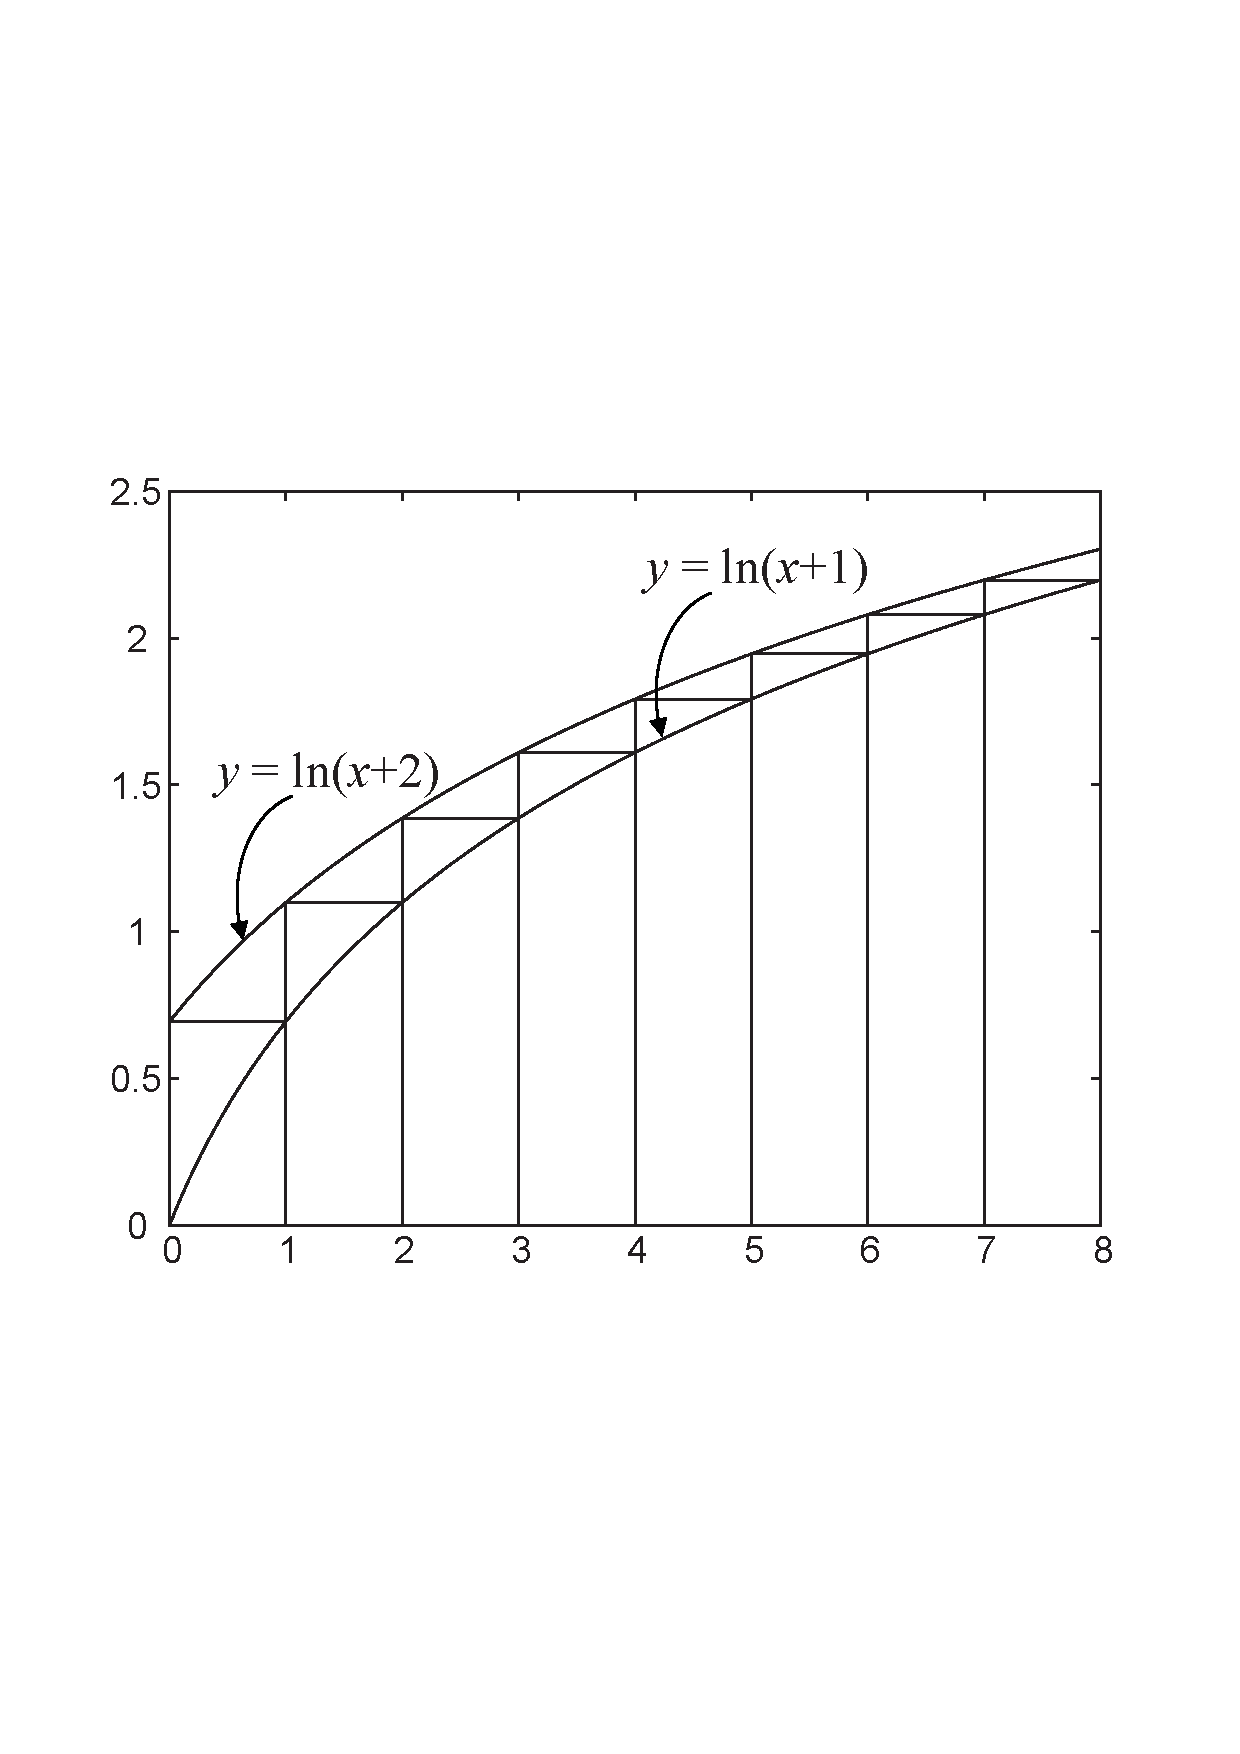
\includegraphics[width=3in,clip]{figures/mq-integral1.pdf}
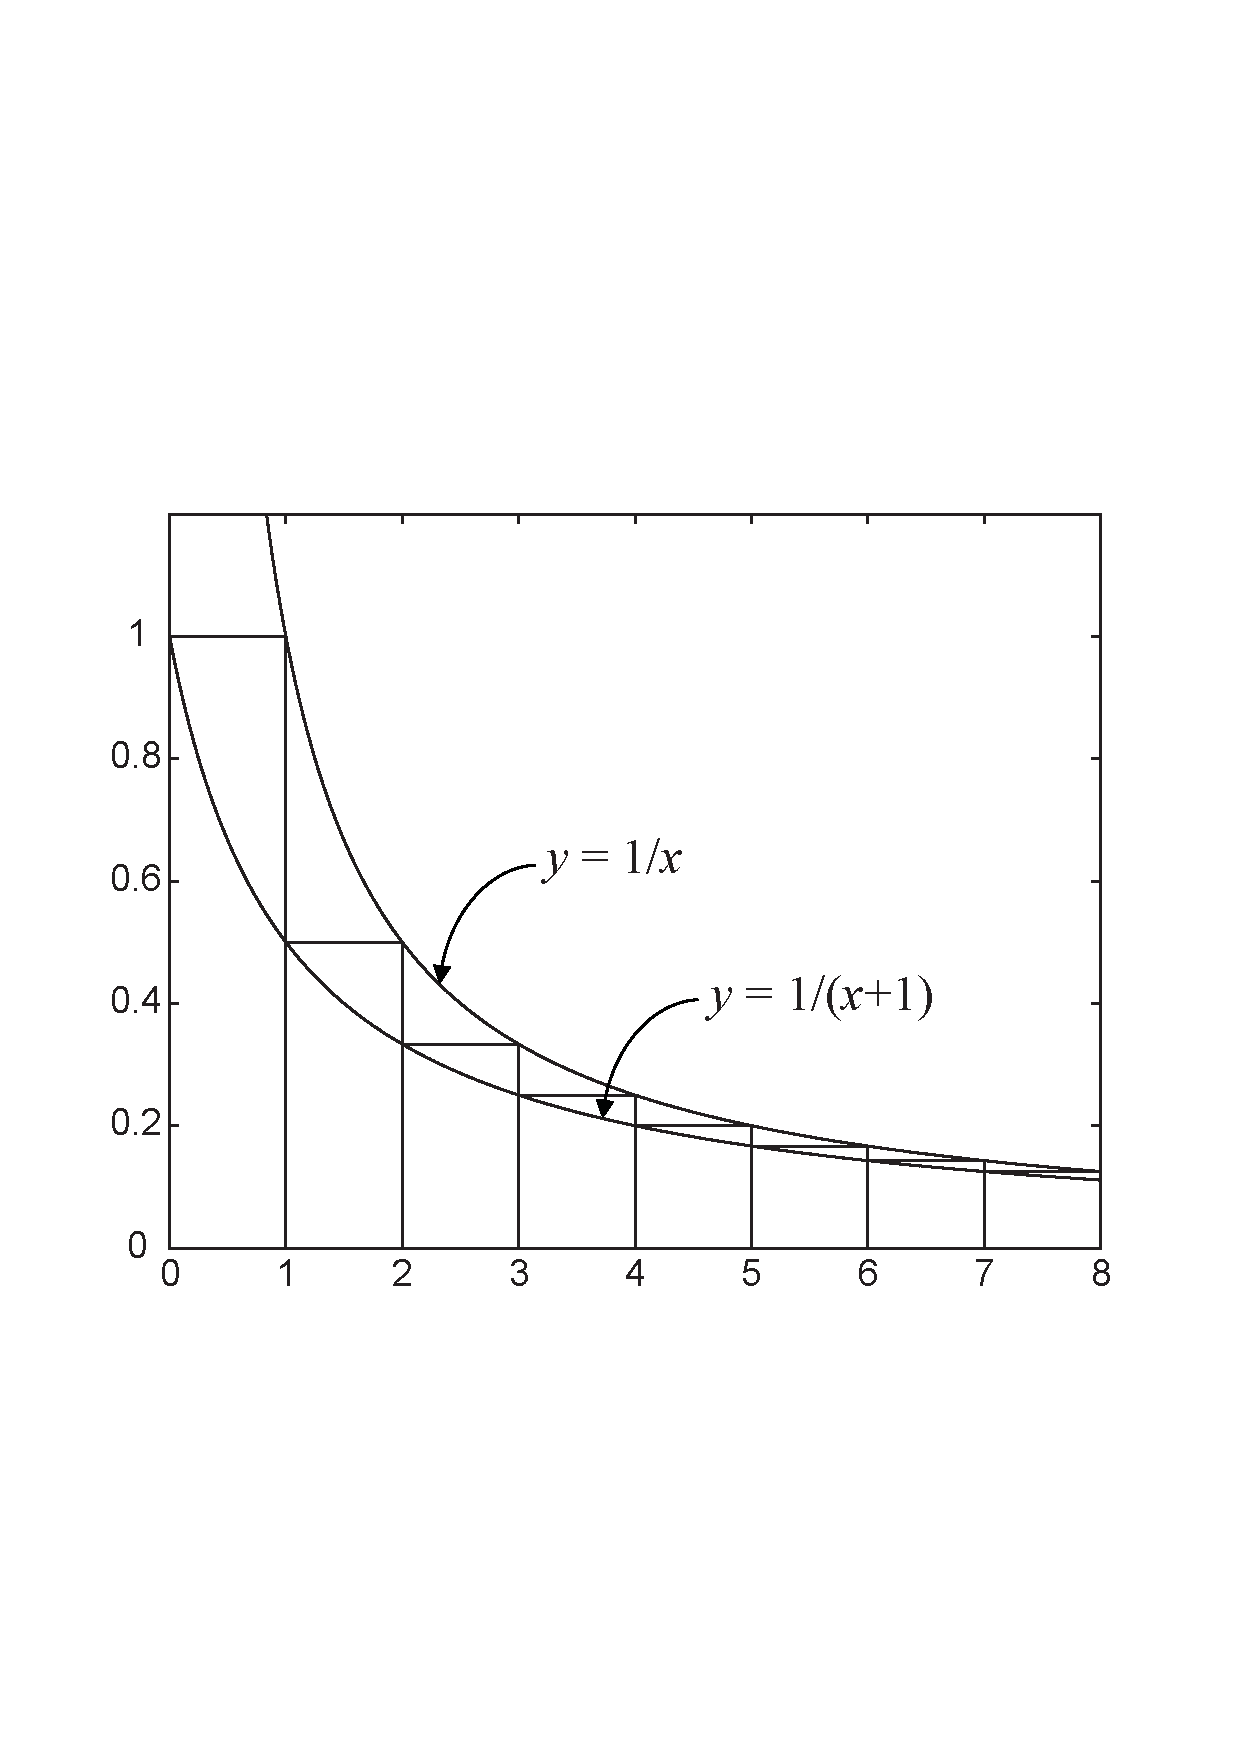
\includegraphics[width=3in,clip]{figures/mq-integral2.pdf}
\end{center}
\end{figure}

\begin{itemize}

\item $\displaystyle \sum_{i=1}^n \ln (i+1) \le \int_0^n \ln(x+2)
dx $

\item $\displaystyle \sum_{i=1}^n \ln (i+1) \le \ln 2 + \int_1^n
\ln(x+1) dx $

\item $\displaystyle \sum_{i=1}^n \frac{1}{i} \ge \int_0^n
\frac{1}{x+1} dx $

%\item $\displaystyle \sum_{i=1}^n \frac{1}{i} \le 1.5 + \int_3^n
%\frac{1}{x} dx $

\end{itemize}

\begin{solution}The 2nd and 3rd inequalities hold.\end{solution}

\end{problem}

%%%%%%%%%%%%%%%%%%%%%%%%%%%%%%%%%%%%%%%%%%%%%%%%%%%%%%%%%%%%%%%%%%%%%
% Problem ends here
%%%%%%%%%%%%%%%%%%%%%%%%%%%%%%%%%%%%%%%%%%%%%%%%%%%%%%%%%%%%%%%%%%%%%
\endinput